\chapter{Grundlagen}\label{ch:technologien}
Im folgenden Kapitel werden zuerst die grundlegenden Konzepte des \textit{Event Stormings} erläutert.
Hierbei wird auf dessen Herkunft und Entwicklung eingegangen.
Neben diesen Grundlagen werden anschließend die für diese Arbeit notwendigen Änderungen und Erweiterungen dargelegt.
Weiterhin werden die wichtigsten Technologien erläutert, welche für die Implementierung der Anwendungen nötig waren.
Um eine bessere Übersicht zu schaffen, sind die Technologien nach dem Anwendungsteil, für welche diese nötig sind, unterteilt.

\section{Event Storming}\label{sec:event-storming}
Dieses Unterkapitel befasst sich mit der Herkunft des \textit{Event Stormings}, dem \ac*{DDD}.
Zudem wird ein klassischer Ablauf eines \textit{Event Stormings} erläutert und daran die Vorteile dieser Methodik für das Requirements Engineering beleuchtet.
Abschließend werden die Änderungen und Erweiterungen, welche im Kontext dieser Arbeit vorgenommen wurden, erklärt.

\subsection{Allgemein}\label{subsec:allgemein}
\todo{Bevor ich dieses und das folgende Unterkapitel schreibe, erst noch mal das~\cite*{dddd} und~\cite*{introES} lesen.}
\begin{itemize}
    \item Alberto Brandolini und das ES
    \item DDD als Grundlage
    \item Wie verläuft so ein ES Workshop (Beschrieben in seinem Buch, mehrfach)
    \item Wichtigsten Eckpunkte
    \item Warum ist es besser als Brain Storming oder ähnliches?
    \item Beispielhaftes Event Storming Board (Bild und beschreibungstext um später darauf bezug nehmen zu können)
\end{itemize}

\subsection{Erweiterung}\label{subsec:erweiterung}
\todo{Hier das vorherige Kapitel abwarten um alle Änderungen/Erweiterungen besser daran fest zu machen.}
\begin{itemize}
    \item Erweiterungen für Wirtschaft (Pages -> daraus generierte Mockups, abgehen von dem "Wir wollen keinen PC benutzen" des ES)
    \item Ideen für die Lehre (Wird in dieser Arbeit nicht näher beleuchtet, da es für den Beleg der Funktionalität nicht mehr möglich ist dies ausreichend in der Bearbeitungszeit zu machen)
    \item ES -> Ablauf von Schritten -> Albert -> Workflow (Arbeitsablauf) beschreibungen -> Mögliche Idee zum besseren Nahebringen von komplexeren Abläufen in Vorlesungen. (Verbildlichung)
\end{itemize}

\section{Technologien}\label{sec:technologien}
Dieses Kapitel gibt einen Überblick über die verwendeten Technologien in der Umsetzung.
Da die Implementierung aus verschiedenen Komponenten besteht, ist dieses Kapitel in drei weitere Unterkapitel aufgeteilt.
Es wird somit getrennt auf die Java Library \textit{fulibWorkflows}, das Spring Boot Backend des \textit{fulibWorkflows Web-Editors}
und das zum Editor dazugehörige Frontend, welches mit Angular umgesetzt wurde.

\subsection{fulibWorkflows}\label{subsec:fulibworkflows}
\textit{fulibWorkflows} ist eine Java Library, welche Arbeitsabläufe, im Folgenden "workflows", in \ac*{YAML}-Syntax notiert als Eingabe nimmt und daraus
sowohl ein Event Storming Board, im workflow beschriebene Mockups und Objekt-/ Klassendiagramme generiert.
Welche Form die YAML-Eingabe haben muss und wie die Dateien aussehen und generiert werden, folgt in einem späteren Kapitel.

\subsubsection{Antlr}\label{subsubsec:antlr}
Antlr bietet die Möglichkeit einen Parser über eine eigens geschriebene Grammatik zu generieren.
Die Grammatik muss Links ableitend sein und ist in EBNF.
\todo{Was bedeutet das?}
Der generierte Parser ermöglicht zudem das Aufbauen und Ablaufen eines \textit{Parse trees}.
Hierdurch ergibt sich die Möglichkeit während dem Parsen weitere Aktionen durchzuführen, welche den späteren Programmablauf eines Tools unterstützen können.

\lstinputlisting[caption={Beispiel einer einfachen Grammatik in Antlr},label={lst:grammar-example}]{listings/AntlrExample.g4}

In Listing~\ref{lst:grammar-example} ist ein Beispiel für eine einfache Grammatik zur Erkennung von mathematischen Gleichungen dargestellt.\cite{antlrOrg}
Hierbei ist es lediglich möglich Zahlen mittels Klammern, Addition, Subtraktion, Multiplikation und Division miteinander zu kombinieren.
Die Länge eines Ausdruckes ist durch den rekursiven Aufbau der Grammatik nicht begrenzt.

\begin{lstlisting}[caption={Einfacher mathematischer Ausdruck},label={lst:mathematical-input}]
    ((199+2324)*43)/55

\end{lstlisting}

Die zuvor beschriebene Grammatik kann mittels weiterer Tools auf eine Eingabe geprüft werden.
Eine zulässige Eingabe für die festgelegte Grammatik aus~\ref{lst:grammar-example} ist in~\ref{lst:mathematical-input} dargestellt.
Die Überprüfung auf die Richtigkeit einer Eingabe oder auch der Grammatik kann über Tools bereits vor einer Generierung von Code durchgeführt werden.
Hierzu wurde das Diagramm aus Abbildung~\ref{fig:parse-example} mittels dem Antlr Plugin für IntelliJ generiert.

\begin{figure}[h]
    \centering
    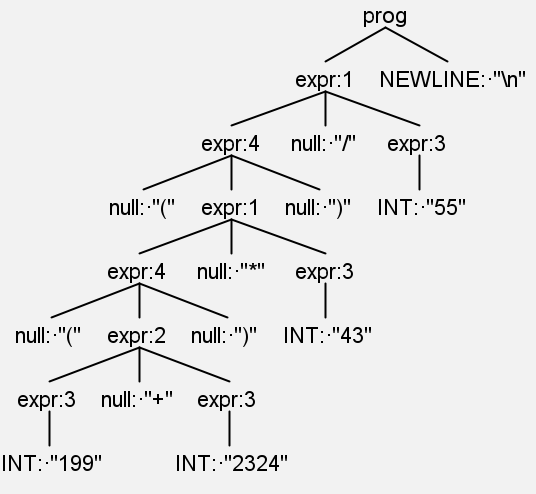
\includegraphics[width=0.3\textwidth]{images/parseTreeExample}
    \caption{ParseTree für einen mathematischen Ausdruck}
    \label{fig:parse-example}
\end{figure}

Hierbei ist ersichtlich, dass die Wurzel bei der obersten Regel \textbf{prog} beginnt und alle weiteren Kindknoten durch verschachtelte \textbf{expr} Regeln kreiert wurden.
Der oberste Teilausdruck ist die Division aus einem komplexeren linken Ausdruck und dem rechten Ausdruck, welcher direkt einer Nummer zugeordnet werden konnte und somit keine weiteren Kindknoten mehr haben kann.
Dies entsteht durch die Unterscheidung bei der Grammatik in Terminale und Nicht-Terminale.
Hierbei werden wie in~\ref{lst:grammar-example} dargestellt Nicht-Terminale Regeln kleingeschrieben und Terminale werden in Großbuchstaben verfasst.
In der vereinfachten Grammatik sind lediglich ganze Zahlen als Eingabe erlaubt.

Dies sind lediglich die Grundlagen von Antlr, auf die genauere Verwendung des generierten Parsers und Besonderheiten der Grammatik wird in~\ref{subsec:fulibworkflows-grammatik} eingegangen.

\subsubsection{String Templates}
\textit{StringTemplate} gehören wir das vorherige Antlr zum \textit{Antlr Project}.
Antlr verwendet ebenfalls String Templates zur Generierung von formatiertem Text, im Folgenden als \textit{Code} bezeichnet.
Templates (übersetzt: Schablone) ermöglichen es zum Beispiel die feste Syntax einer Programmiersprache wie Java mit variablen Werten für
Variablen, Klassen, Methoden, also den generellen Bausteinen einer Sprache zu füllen.
Durch diese Funktionalität bieten sich String Templates sehr gut zu Generierung von Dateien an.
Ursprünglich ist \textit{StringTemplate} eine Java Library, jedoch wurden bereits Portierungen für C#, Objective-C, JavaScript und Scala erstellt.

Die folgenden Erläuterungen beziehen sich auf die Java Library von \textit{StringTemplate}, da diese in dieser Arbeit verwendet wurde.
Die einfachste Möglichkeit für die Verwendung eines String Templates ist in Listing~\ref{lst:simpleTemplate} zu sehen.

\lstinputlisting[caption={``Hello World!'' - Beispiel mittels StringTemplate},label={lst:simpleTemplate}, language=Java]{listings/JavaStringTemplateExample.java}

Die Klasse \textit{ST} aus Zeile 3 kann mit einem String initialisiert werden.
In diesem Beispiel wurden als Begrenzer für das zu ersetzende Stück des Textes \textit{<>} verwendet.
Im Anschluss wird dem neuen \textit{ST} Objekt mithilfe der add()-Methode ein bestimmter Wert hinzugefügt.
Der erste Parameter der Methode ist der Bezeichner innerhalb eines Templates, zu beachten ist die Angabe des Bezeichners ohne die Begrenzer.
Der eigentliche Wert wird als zweiter Parameter übergeben und besitzt in diesem Beispiel den Text \textbf{World}.
Um nun den fertig ersetzten Text aus dem Template und dem übergebenem Wert zu bekommen, muss auf dem \textit{ST} Objekt die Methode render() aufgerufen werden.
Hierbei werden die Platzhalter des Templates durch den zuvor übergebenen Wert ersetzt und als String zurückgegeben.
In Zeile 6 wird nun abschließend der fertige Text auf der Konsole ausgegeben, `Hello, World!`.
Dieses Beispiel entstammt der offiziellen Webseite von \textit{StringTemplate}.\cite*{stOrg}

Für ein strukturiertes Arbeiten mit vielen Templates bietet \textit{StringTemplate} die Möglichkeit StringTemplateGroups zu erstellen.
Hierbei können mehrere Templates in einer Datei beschrieben werden um aufeinander aufbauende Templates nicht im Code, sondern einer gesonderten Datei zu organisieren.
In diesen Dateien, welche die Dateiendung \textbf{.stg} tragen, können die Begrenzer (eng.: Delimiters) frei gewählt werden.
Dies ist je nach Kontext des Templates nötig, da zum Beispiel die Generierung von HTML-Dateien, welche \textit{<>} als Zeichen zum Abgrenzen von Bereichen verwenden.
Bei der Wahl der Begrenzer sollte somit stets auf die Wahl der Zeichen im Kontext der zu generierenden Sprache geachtet werden.
Zum Parsen einer StringTemplateGroup wurde ein mit Antlr generierter Parser verwendet.\cite*{stgParser}

\lstinputlisting[caption={Beispiel einer .stg-Datei},label={lst:stgFile}]{listings/Example.stg}

Wie zuvor beschrieben ist in Listing~\ref{lst:stgFile} zu erkennen, dass in Zeile 1 die Begrenzer auf \textit{{}} gesetzt wurden.
Dies hat den Hintergrund, dass in diesem Beispiel ein Text in eine HTML-Datei generiert werden soll.
Hierfür könnten auch die Standardbegrenzer verwendet werden, allerdings müsste dann anstelle von \textbf{<span>} \textbf{\<span\>} stehen.
Da dies für HTML-Dateien allerdings einen immensen Aufwand bedeutet, macht die Nutzung anderer Begrenzer Sinn.
In Zeile 3 werden für ein StringTemplate, sowohl der Name des Templates, als auch Übergabeparameter definiert werden.
Ein StringTemplate wird durch \textit{>>} geschlossen und das nächste Template könnte definiert werden.
Die Begrenzer in Zeile 5 zeigen, dass alles, was sich zwischen Ihnen befindet, einen Übergabeparameter in sich trägt.
Somit ist das Wiederverwenden des Templates und die variable Befüllung gewährleistet.

Um diese Templates nun in einem Java Programm zu verwenden, benötigt es unter anderem die zuvor beschriebenen ST Klasse, sowie
die Klasse \textit{STGroupFile}, welche für die Verwaltung der stg-Datei als auch deren Templates benötigt wird.
In Zeile 6 von Listing~\ref{lst:stgJavaFile} ist zu erkennen, dass einem STGroupFile Objekt bei der Initialisierung eine URL übergeben werden muss.
Diese URL verweist auf die stg-Datei.
Im Anschluss kann, wie in Zeile 8 ersichtlich, über die getInstanceOf()-Methode auf ein bestimmtes Template in der stg-Datei zugegriffen werden.
Hierbei ist es wichtig, keine Fehler bei der Benennung zu machen.
Schließlich ist die weiterführende Verwendung bereits zuvor mittels der ST-Klasse beschrieben worden.

\lstinputlisting[caption={Nutzung einer STG-Datei in Java},label={lst:stgJavaFile}]{listings/JavaSTGExample.java}

Bei der Ausführung dieses Beispieles würde auf der Konsole der Text aus Listing~\ref{lst:outputSTG} angezeigt werden.

\begin{lstlisting}[label={lst:outputSTG}]
<span>
    This test about the university is written in english.
</span>
\end{lstlisting}

\subsubsection{JSON-Schema}\label{subsubsec:json-schema}
Bei einem JSON-Schema kann man die erlaubten Eingaben eines Nutzers, sowohl für JSON-Dateien als
auch YAML-Dateien beschränken.

\todo Welche Version?, Schemastore.org, wie funst das mit den schemas?

Durch ein fest definiertes Schema ist es vielen IDEs, darunter auch IntelliJ und VSCode, welche
aus einem Schema nicht nur die fertige Datei auf Fehler überprüfen, sondern dem Entwickelnden bereits
zum Zeitpunkt des Schreibens einer Datei mittels Autovervollständigung unterstützen kann.
Eine Liste aller IDEs, welche diesen support mittels schemastore unterstützen sind unter folgendem
Link zu finden: \url{https://www.schemastore.org/json/#editors}

\subsubsection{fulibTools}
\todo
Dank fulibTools ist auch fulib mit drin.
FulibTools ist zur Generierung von Objektidiagrammen genutzt worden.
Fulib (Bei FulibTools mit integriert) zur Generierung von Klassendiagrammen.

\subsection{fulibWorkflows Web-Editor FE}\label{subsec:fulibworkflows-web-editor}
\todo
Da brauchte es etwas mehr als beim BE\@.
Die Entscheidungen für die verwendeten Technologien im Frontend wurden aufgrund
der Idee der Integrierung vom Editor auf fulib.org getroffen.

\subsubsection{Angular}
\todo
Wir kennen es.
Wir lieben es.

\subsubsection{Bootstrap}
\todo
Alles für den Dackel, alles für den Club unser Leben für die schön gestylten FEs.
Simpel, oder?
Ja, okay.
Man nutzt dann auch ng-bootstrap für Angular Anwendungen.
Natürlich auch noch bootstrap-icons.
Will ja niemand traurig machen und von Adrian verdroschen werden.

\subsubsection{Codemirror}
\todo
Schönes Ding.
Ngx-codemirror ist es dann speziell für eine Angular Anwendung geworden.
Eigentlich alles out of the box benutzt.

\subsubsection{Angular-split}
\todo
Find ich schon gut zu erwähnen.
Ohne die geile dependency wäre das FE nie so pornös geworden.

\subsubsection{file-saver}
\todo
Weitere erwähnenswerte dependency.
Wird genutzt um Dateien, die vom BE kommen, auch herunterladen zu können.

\subsubsection{ajv}
\todo

\subsubsection{js-yaml}
\todo


\subsection{fulibWorkflows Web-Editor BE}\label{subsubsec:backend}
\todo
Yeey alle Technologien die ich im Backend benutzt habe.

\subsubsection{Spring Boot}
\todo
Framework mit dem man easy mal ein backend generiert bekommt.
Durch Java und viele Dependency allerdings alles andere als ein leichtgewicht.

Dennoch musste ein Java backend her, da sonst fulibWorkflows nicht hätte integriert werden können.
Jedenfalls nicht ohne noch mehr middle ware.

Zudem hatte ich im Praktikum mit Spring Boot Erfahrungen gesammelt.
Die Verwendung von Annotations und dem aufsplitten zwischen Controller und Service ist mir bereits
durch Nest.js bekannt gewesen.

Dennoch muss man sagen, dass durch die von Spring Boot bereits integrierten libraries nichts weiter
außer fulibWorkflows hinzugefügt werden musste.
Immerhin umfasst der Code vom Backend vielleicht 300 Lines of Code.

\subsubsection{fulibWorkflows}
\todo
Sollte mindestens irgendwo erwähnt werden.
Kann man ggf. auch in dem Text zum Kapitel schreiben.

\subsection{Deployment}\label{subsec:deployment}
\todo
Ein Web Editor will natürlich für alle erreichbar sein.
Und fulibWorkflows muss auch irgendwo bereitgestellt werden, damit es das Backend und alle anderen
interessierten benutzen können.

\subsubsection{MavenCentral}\label{subsubsec:mavencentral}
\todo
MavenCentral ein wirklicher Hussarones was das publishen angeht.
Glücklicherweise ist fulibWorkflows Teil der Fujaba Tool Suite, wodurch die benötigten
Zugriffsrechte bereits vorhanden und andere Libraries bereits gepublished wurden.
Hierdurch war es recht schnell möglich mit dem zuvor erworbenem Wissen fulibWorkflows
zu publishen.

\subsubsection{Heroku}\label{subsubsec:heroku}
\todo
Der Web-Editor soll immer erreichbar sein.
Dies ist durch Heroku nur bedingt möglich.
Heroku bietet allerlei Möglichkeiten verschiedenste Anwendungen bereitzustellen.
Auch mit einem kostenlosen Plan ist es ohne Probleme möglich solch kleine Anwendungen bereitzustellen.

FE Deployment war easy, auch wenn ich erstmal wieder in eins meiner früheren Projekte gucken musste.
BE Deployment war kniffliger, doch man ist nie der erste der eine Spring Boot application
auf Heroku deployen will.
Daher Tutorial reingefahren und ab ging der gebutterte Lachs.
